

\begin{table}[h]\begin{tabular}{|>{\columncolor[gray]{0.9}} p{3cm}|p{2.8cm}|p{2.8cm}|p{2.8cm}|c|}
    \hline
    \rowcolor[gray]{.9}
    Path finding & Isolated Worms matching & Cluster Worms matching 
    & Total Matching 
    & Time (s) \\ 
    \hline  
    Every Path (me) & 8/8 (100\%) & 7/25 (28\%) & 15/33 (45.4\%) & 21.8 \\ 
    \hline
    P.Guessing (me) & 8/8 (100\%) & 10/25 (40\%) & 18/33 (54.5\%) & 23.7\\
    \hline
    Every Path & 8/8 (100\%)& 15/23 (65.2\%) & 23/33 (69.7\%)& 42.3 \\
    \hline
    P.Guessing & 8/8 (100\%)& 21/25 (84\%) & 29/33 (87.8\%) & 45 \\
    \hline
  \end{tabular}
  \label{tab1}
  \caption{Results of automatic worm shape matching on test image}
\end{table}

\begin{figure}[h t b p ! H]
  \centering
  \subfloat[Original Image]{\label{ori2}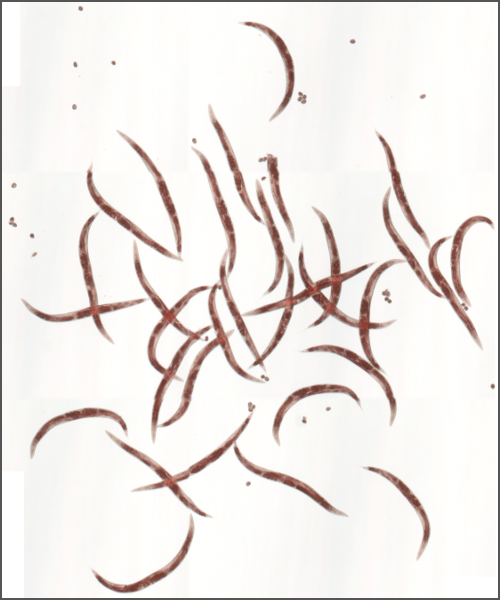
\includegraphics[scale=0.3]{results/test2/original2}}
\qquad
  \subfloat[Binary Image]{\label{bin2}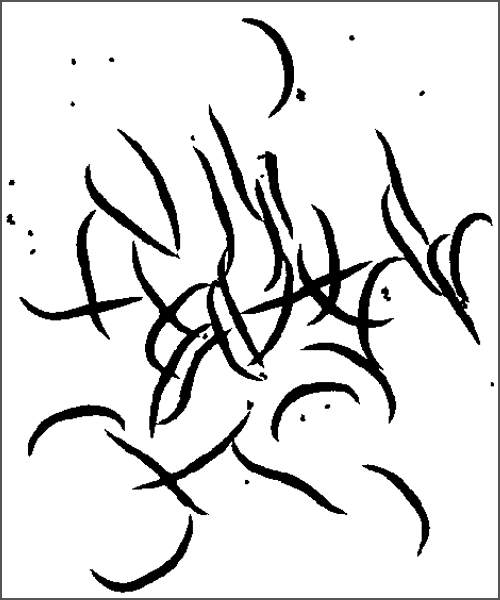
\includegraphics[scale=0.3]{results/test2/binary2}}
\qquad
  \subfloat[Distance map]{\label{dtshape2}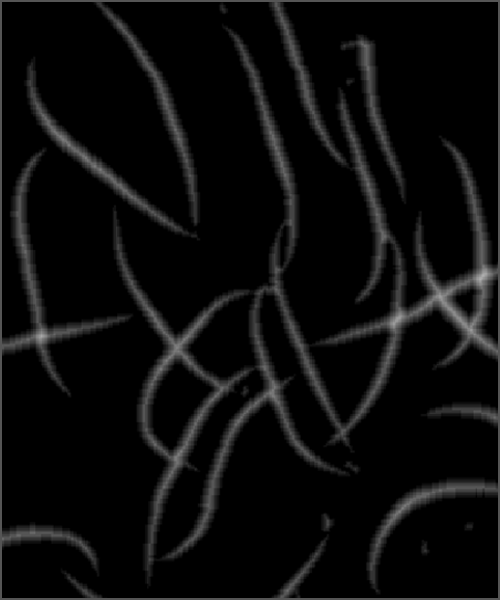
\includegraphics[scale=0.3]{results/test2/dt2}}
\qquad
  \subfloat[Shape skeleton]{\label{skeleton2}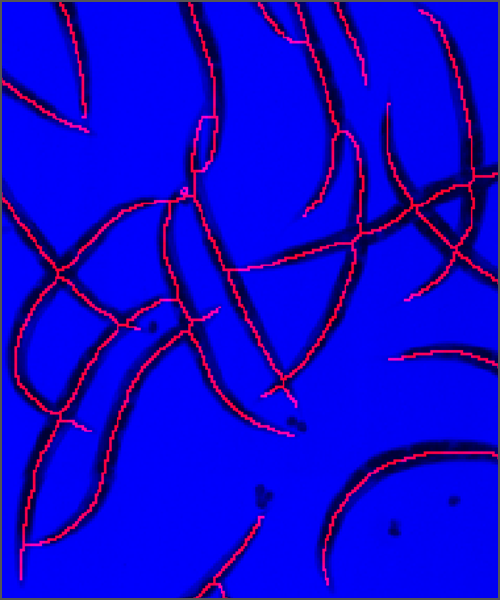
\includegraphics[scale=0.3]{results/test2/skeleton-frame}}
\qquad
  \subfloat[Segmentation in Clusters]{\label{clust2}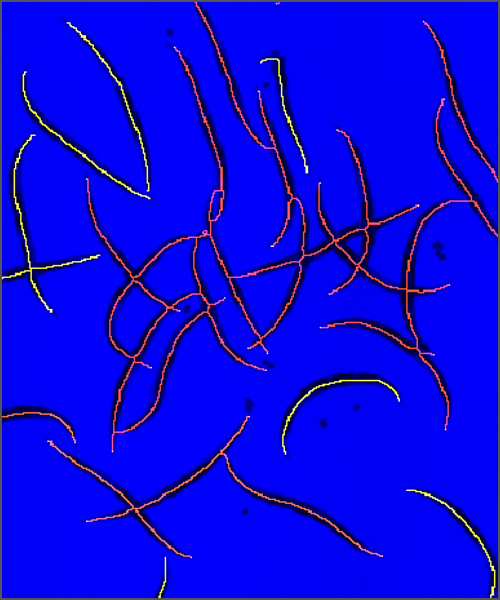
\includegraphics[scale=0.3]{results/test2/cluster2}}
\qquad
  \subfloat[Isolated Worm Profiling]{\label{prof2}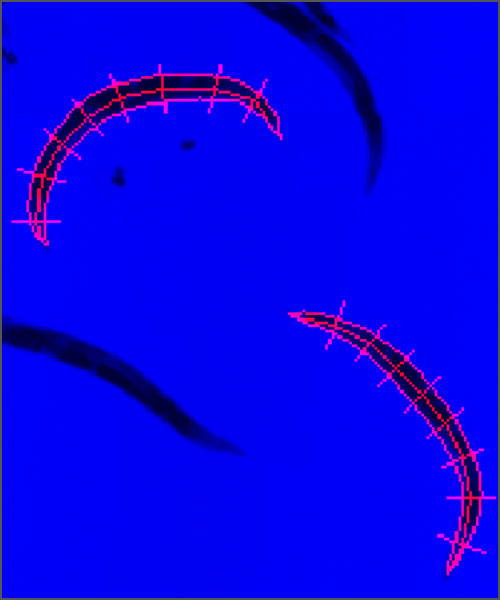
\includegraphics[scale=0.3]{results/test2/wprof2}}
  \caption{Sequence of image processing steps before shape matching on test image 2}
\end{figure}


\begin{figure}[h t b p ! H]
  \centering
  \subfloat[Skeleton with missing endpoints]{\label{ori2}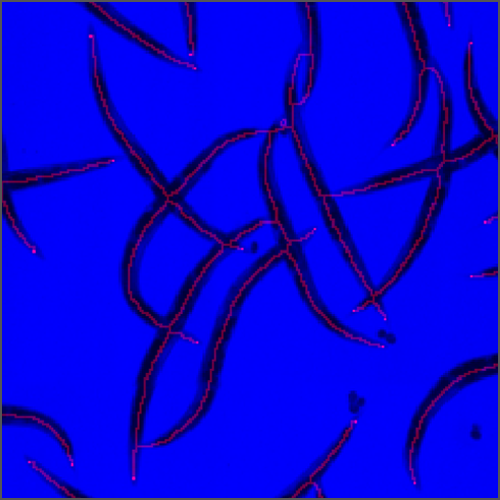
\includegraphics[scale=0.4]{results/test2/skeleton-zoom2}}
\qquad
  \subfloat[Skeleton after addition of missing endpoints]{\label{bin2}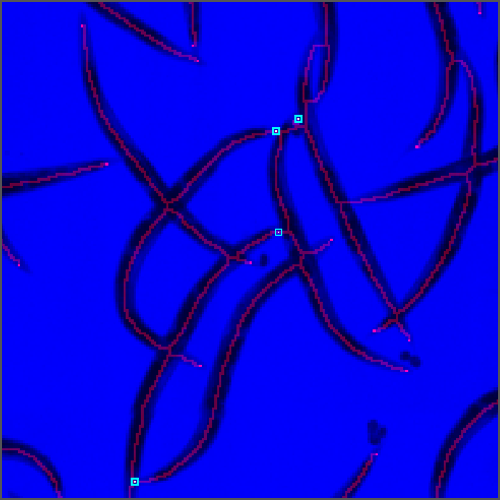
\includegraphics[scale=0.4]{results/test2/skeleton-zoomEnd2}}
\end{figure}


